\documentclass[11pt,a4paper]{article}

\usepackage[T1]{fontenc}
\usepackage[margin=1in]{geometry}
\usepackage{amsmath}
\usepackage{amssymb}
\usepackage{array}
\usepackage{booktabs}
\usepackage{xcolor}
\usepackage{tikz}
\usetikzlibrary{arrows.meta,positioning,calc,fit}

\title{ELEC5803 HLS Exam Study\\Step-by-Step Solution to Question 5}
\author{}
\date{}

\tikzset{
  >={Latex[length=2mm]},
  block/.style={draw, rounded corners, minimum width=2.2cm, minimum height=0.9cm, align=center},
  mac/.style={draw, rounded corners, fill=green!8, minimum width=2.4cm, minimum height=1cm, align=center},
  vote/.style={draw, rounded corners, fill=orange!12, minimum width=2cm, minimum height=0.9cm, align=center},
  mem/.style={draw, rounded corners, fill=blue!8, minimum width=2cm, minimum height=0.9cm, align=center},
}

\begin{document}
\maketitle

\section*{Course-slide basis}
This solution follows the redundancy and reliability discussion in
\texttt{Slides/ELEC5803\_Slides10\_Testability and Dependability\_AA2.pdf}, especially the matrix-multiplication example, DMR/TMR/NMR, temporal redundancy, and information redundancy sections.

\section*{1. Interpreting the problem}
The matrices have dimensions
\[
A\in \mathbb{R}^{3\times 4},\qquad B\in \mathbb{R}^{4\times 3},\qquad C=AB\in \mathbb{R}^{3\times 3}.
\]
So the output matrix has
\[
3\times 3=9
\]
elements. The question explicitly says:
\begin{itemize}
  \item each output element computation is treated as one \emph{operation},
  \item the MAC is the computation module,
  \item the fault process follows a Poisson model with average rate $\lambda$.
\end{itemize}

Therefore, if one operation takes time $t$, then from the slide figure:
\[
P_{\text{ne}}(t)=e^{-\lambda t},\qquad
P_{\text{error}}(t)=1-e^{-\lambda t}.
\]
For compactness, define
\[
q=P_{\text{ne}}(t)=e^{-\lambda t},\qquad p=P_{\text{error}}(t)=1-e^{-\lambda t}.
\]

\section*{2. Part (a): DMR and TMR}
\subsection*{2.1 Baseline single-module system}
With one MAC module, the probability that an operation finishes without error is
\[
q=e^{-\lambda t},
\]
and the probability that the operation is erroneous is
\[
p=1-e^{-\lambda t}.
\]

\subsection*{2.2 Dual Modular Redundancy (DMR)}
DMR duplicates the computation and compares the two outputs.

\begin{figure}[h!]
\centering
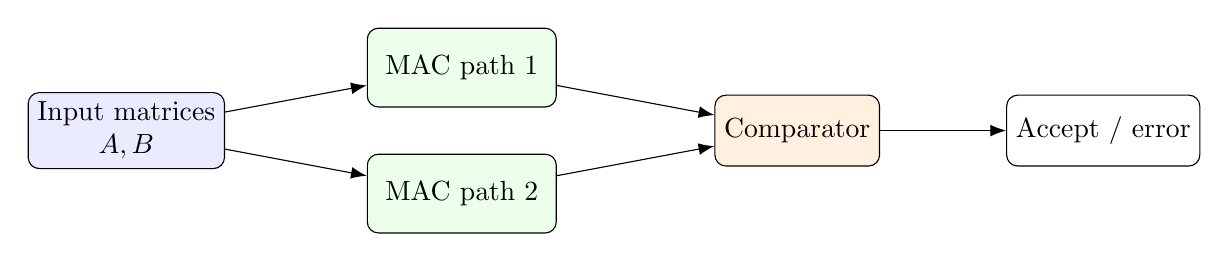
\begin{tikzpicture}[node distance=8mm and 12mm]
  \node[mem] (in) {Input matrices\\$A,B$};
  \node[mac, right=18mm of in, yshift=8mm] (m1) {MAC path 1};
  \node[mac, right=18mm of in, yshift=-8mm] (m2) {MAC path 2};
  \node[vote, right=20mm of m1, yshift=-8mm] (cmp) {Comparator};
  \node[block, right=16mm of cmp] (out) {Accept / error};
  \draw[->] (in) -- (m1);
  \draw[->] (in) -- (m2);
  \draw[->] (m1) -- (cmp);
  \draw[->] (m2) -- (cmp);
  \draw[->] (cmp) -- (out);
\end{tikzpicture}
\caption{DMR for one matrix-element computation.}
\end{figure}

DMR is mainly an \textbf{error-detection} scheme. If at least one module is faulty, the DMR system is considered to have encountered an error/failure event for that computation.

Hence the probability of DMR error is:
\[
P_{\text{DMR,error}}
=1-q^2
=1-e^{-2\lambda t}.
\]
Equivalently,
\[
P_{\text{DMR,error}}=2pq+p^2.
\]

\paragraph{Interpretation:}
\begin{itemize}
  \item $2pq$: exactly one module is erroneous,
  \item $p^2$: both modules are erroneous.
\end{itemize}

\subsection*{2.3 Triple Modular Redundancy (TMR)}
TMR uses three replicated modules and a 2-out-of-3 majority voter.

\begin{figure}[h!]
\centering
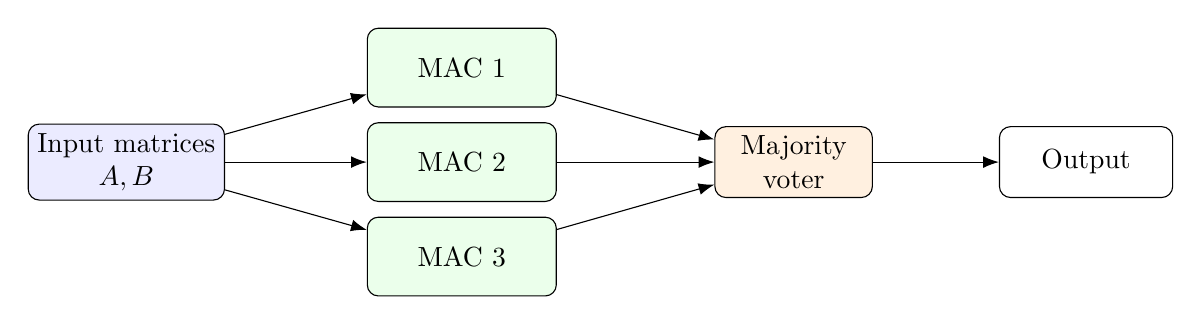
\begin{tikzpicture}[node distance=8mm and 12mm]
  \node[mem] (in) {Input matrices\\$A,B$};
  \node[mac, right=18mm of in, yshift=12mm] (m1) {MAC 1};
  \node[mac, right=18mm of in] (m2) {MAC 2};
  \node[mac, right=18mm of in, yshift=-12mm] (m3) {MAC 3};
  \node[vote, right=20mm of m2] (maj) {Majority\\voter};
  \node[block, right=16mm of maj] (out) {Output};
  \draw[->] (in) -- (m1);
  \draw[->] (in) -- (m2);
  \draw[->] (in) -- (m3);
  \draw[->] (m1) -- (maj);
  \draw[->] (m2) -- (maj);
  \draw[->] (m3) -- (maj);
  \draw[->] (maj) -- (out);
\end{tikzpicture}
\caption{TMR for one matrix-element computation.}
\end{figure}

From the slides, the TMR error probability is
\[
P_{\text{TMR,error}} = 3p^2q + p^3.
\]

\paragraph{Why?}
The TMR output is wrong only if:
\begin{itemize}
  \item any two of the three modules are erroneous, or
  \item all three modules are erroneous.
\end{itemize}

So
\[
P_{\text{TMR,error}}
= \binom{3}{2}p^2q + \binom{3}{3}p^3
= 3p^2q + p^3.
\]
Substituting $p=1-e^{-\lambda t}$ and $q=e^{-\lambda t}$:
\[
\boxed{
P_{\text{TMR,error}}
=3(1-e^{-\lambda t})^2e^{-\lambda t} + (1-e^{-\lambda t})^3.
}
\]

\subsection*{2.4 Final answer for part (a)}
\[
\boxed{
P_{\text{DMR,error}}=2pq+p^2=1-e^{-2\lambda t}
}
\]
\[
\boxed{
P_{\text{TMR,error}}=3p^2q+p^3
}
\]
with
\[
p=1-e^{-\lambda t},\qquad q=e^{-\lambda t}.
\]

\section*{3. Part (b): NMR, N-temporal redundancy, and information redundancy}
\subsection*{3.1 N-Modular Redundancy (NMR)}
This generalizes TMR to $N$ replicated modules with a $k$-out-of-$N$ voter.

\begin{figure}[h!]
\centering
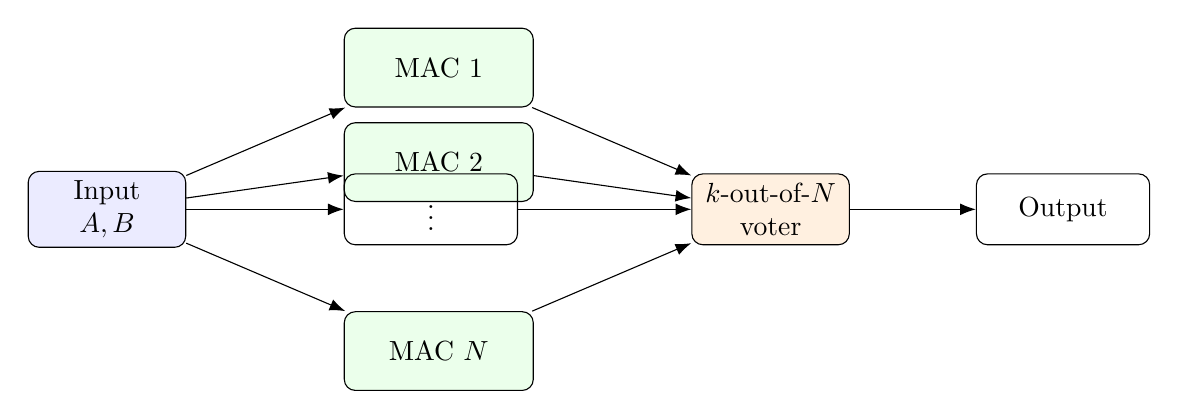
\begin{tikzpicture}[node distance=7mm and 10mm]
  \node[mem] (in) {Input\\$A,B$};
  \node[mac, right=20mm of in, yshift=18mm] (m1) {MAC 1};
  \node[mac, right=20mm of in, yshift=6mm] (m2) {MAC 2};
  \node[block, right=20mm of in] (dots) {$\vdots$};
  \node[mac, right=20mm of in, yshift=-18mm] (mn) {MAC $N$};
  \node[vote, right=22mm of dots] (vote) {$k$-out-of-$N$\\voter};
  \node[block, right=16mm of vote] (out) {Output};
  \draw[->] (in) -- (m1);
  \draw[->] (in) -- (m2);
  \draw[->] (in) -- (dots);
  \draw[->] (in) -- (mn);
  \draw[->] (m1) -- (vote);
  \draw[->] (m2) -- (vote);
  \draw[->] (dots) -- (vote);
  \draw[->] (mn) -- (vote);
  \draw[->] (vote) -- (out);
\end{tikzpicture}
\caption{Generalized NMR ($k$-out-of-$N$) architecture.}
\end{figure}

If the system is correct when at least $k$ modules are fault-free, then the error probability is:
\[
\boxed{
P_{\text{NMR,error}}
=
\sum_{i=N-k+1}^{N}\binom{N}{i}p^i q^{N-i}.
}
\]
For TMR, $N=3$ and $k=2$, which reduces to $3p^2q+p^3$.

\subsection*{3.2 N-Temporal redundancy}
Temporal redundancy reuses the same hardware $N$ times over time instead of replicating hardware spatially.

\begin{figure}[h!]
\centering
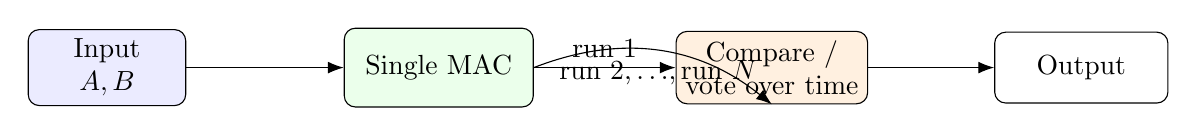
\begin{tikzpicture}[node distance=8mm and 12mm]
  \node[mem] (in) {Input\\$A,B$};
  \node[mac, right=20mm of in] (mac) {Single MAC};
  \node[vote, right=18mm of mac] (check) {Compare /\\vote over time};
  \node[block, right=16mm of check] (out) {Output};
  \draw[->] (in) -- (mac);
  \draw[->] (mac) -- node[above] {run 1} (check);
  \draw[->] (mac.east) to[bend left=30] node[below] {run 2,\,$\ldots$,\,run $N$} (check.south);
  \draw[->] (check) -- (out);
\end{tikzpicture}
\caption{N-temporal redundancy: repeated evaluation on the same MAC hardware.}
\end{figure}

Here:
\begin{itemize}
  \item area overhead is small,
  \item time overhead is high because the same operation is repeated $N$ times,
  \item timing becomes less deterministic, exactly as noted in the slides.
\end{itemize}

\subsection*{3.3 Information redundancy}
Information redundancy augments the operands with checksums.

For the present $3\times 4$ by $4\times 3$ multiplication:
\begin{itemize}
  \item original output size: $3\times 3 = 9$ operations,
  \item checksum-augmented output size: $(3+1)\times(3+1)=4\times 4 = 16$ operations.
\end{itemize}

\begin{figure}[h!]
\centering
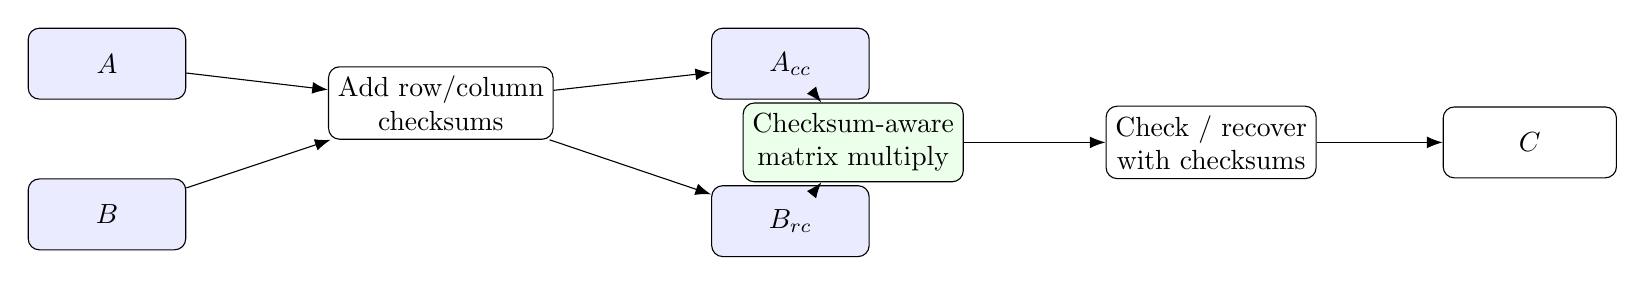
\begin{tikzpicture}[node distance=10mm and 12mm]
  \node[mem] (a) {$A$};
  \node[mem, below=10mm of a] (b) {$B$};
  \node[block, right=18mm of a, yshift=-5mm] (aug) {Add row/column\\checksums};
  \node[mem, right=20mm of aug, yshift=5mm] (acc) {$A_{cc}$};
  \node[mem, right=20mm of aug, yshift=-15mm] (brc) {$B_{rc}$};
  \node[mac, right=24mm of aug, yshift=-5mm] (mm) {Checksum-aware\\matrix multiply};
  \node[block, right=18mm of mm] (chk) {Check / recover\\with checksums};
  \node[block, right=16mm of chk] (out) {$C$};
  \draw[->] (a) -- (aug);
  \draw[->] (b) -- (aug);
  \draw[->] (aug) -- (acc);
  \draw[->] (aug) -- (brc);
  \draw[->] (acc) -- (mm);
  \draw[->] (brc) -- (mm);
  \draw[->] (mm) -- (chk);
  \draw[->] (chk) -- (out);
\end{tikzpicture}
\caption{Information redundancy by checksum augmentation.}
\end{figure}

\subsection*{3.4 Comparison table}
\begin{center}
\begin{tabular}{>{\raggedright\arraybackslash}p{3cm} >{\raggedright\arraybackslash}p{3.2cm} >{\raggedright\arraybackslash}p{3cm} >{\raggedright\arraybackslash}p{3.2cm}}
\toprule
Method & Area cost & Time cost & Power / energy trend \\
\midrule
NMR & High; about $N\times$ compute hardware plus voter & Low extra time; usually near-baseline latency with small voting overhead & High instantaneous power and thermal stress due to parallel replicas \\
N-temporal redundancy & Low area; one compute module reused & High; roughly $N\times$ execution time & Lower instantaneous power than NMR, but higher total energy because work is repeated \\
Information redundancy & Moderate; checksum logic and extra storage & Deterministic overhead; for this case 16 operations instead of 9 & Moderate increase because extra checksum operations are computed \\
\bottomrule
\end{tabular}
\end{center}

\subsection*{3.5 Short discussion}
This matches the slides:
\begin{itemize}
  \item \textbf{spatial redundancy} improves functional reliability but increases area, power, and thermal stress,
  \item \textbf{temporal redundancy} saves area but hurts timing reliability because execution time increases,
  \item \textbf{information redundancy} adds deterministic computational overhead through checksum processing.
\end{itemize}

\section*{4. Part (c): combining methods for lower cost and higher reliability}
The best practical design is usually \emph{hybrid}, not purely one technique.

\subsection*{4.1 Reasonable hybrid strategy}
A low-cost and reliable redesign for the matrix multiplier could be:
\begin{itemize}
  \item use \textbf{information redundancy} (checksums) globally to detect most computation errors at moderate cost,
  \item use \textbf{selective TMR} only for the most critical blocks, such as the voter, control logic, or the MAC datapath if the application is safety-critical,
  \item use \textbf{temporal re-execution} only after checksum mismatch is detected, instead of repeating every computation all the time,
  \item optionally keep a \textbf{cold spare} MAC for recovery without permanently paying full thermal cost.
\end{itemize}

\subsection*{4.2 Why this is better}
This hybrid approach reduces cost because:
\begin{itemize}
  \item full NMR everywhere is expensive in area and power,
  \item pure temporal redundancy is too slow,
  \item pure information redundancy detects well but does not always mask errors by itself.
\end{itemize}

By combining them:
\begin{itemize}
  \item checksums provide cheap error detection,
  \item selective spatial redundancy protects only the highest-risk logic,
  \item temporal retry is activated only when needed.
\end{itemize}

So the resulting system achieves:
\begin{itemize}
  \item better functional reliability than using only one light-weight method,
  \item lower area and power than full TMR/NMR everywhere,
  \item lower average execution-time penalty than always-on temporal redundancy.
\end{itemize}

\section*{5. Final exam-style answers}
\subsection*{(a)}
Let
\[
p=1-e^{-\lambda t},\qquad q=e^{-\lambda t}.
\]
Then:
\[
\boxed{P_{\text{DMR,error}}=2pq+p^2=1-e^{-2\lambda t}}
\]
\[
\boxed{P_{\text{TMR,error}}=3p^2q+p^3}
\]

\subsection*{(b)}
\begin{itemize}
  \item NMR: replicate hardware spatially and use a $k$-out-of-$N$ voter.
  \item N-temporal redundancy: repeat the same computation $N$ times on the same MAC.
  \item Information redundancy: augment matrices with row/column checksums and verify the output.
\end{itemize}
For the given case, information redundancy increases the number of matrix-element operations from $9$ to $16$.

\subsection*{(c)}
Use a hybrid design:
\begin{itemize}
  \item checksum-based information redundancy for cheap global detection,
  \item selective TMR/NMR only on the most critical modules,
  \item temporal retry only on detected failures,
  \item optional cold spares for lifetime reliability.
\end{itemize}

\end{document}
